\part{The language}\label{part:zilch}

\chapter{Introduction}\label{chap:zilch-introduction}

Low-level programming is programming with a few abstractions over the hardware.
For example, assembly languages mostly provide no or very little abstractions over CPU instructions (having one instruction set per target).
Functional programming is a kind of programming focused around functions and their composition.
However, because of this, many functional programming languages have a tendancy to be quite slow, at least compared to ``ordinary'' imperative programming languages.

\href{http://www.ats-lang.org/}{ATS} is one of those programming languages claiming to be both functional and quite low-level.
It compiles to C (therefore has a free FFI), has a complex dependent type system and many other things making it kind of great.
But ATS is hard to learn, because it has so much stuff\ldots

Yet Zilch is also a low-level functional programming language.
But the goal is to design a not-so-hard to learn programming language, while still having strong guarantees about the code written\footnote{When this was written, Zilch was far from production-ready, so most
of the guarantees have not yet been described here.}.
Prior knowledge about ML-style programming is still recommended before trying to tackle Zilch, but anybody without this kind of knowledge should also be able to learn Zilch fairly easily.

This part will try to describe and formalize (at least a bit, but some parts may be left informal) the Zilch programming language, going from the usual syntax onto the operational semantics.
Implementation details (such as error messages, program optimisations, \ldots) will not be covered by this document.

\section*{Some notes on the notation used}\label{sec:zilch-introduction-notation}

Zilch is really not a small programming language.
Because of that, sometimes we need some specific notation to described things like inference rules.

The mainly used notation is described here, but not necessarily everything will be described (sometimes, a little bit of common sense helps to understand).

\begin{itemize}
  \item Grammar
        \begin{figure}[H]
          \centering
          \scalebox{.5}{
            
\includegraphics{grammar-template-2}
          }
        \end{figure}
        \begin{itemize}
          \item Sharp rectangles describe that another rule is to be used there (the name of the rule is given in the rectangle);
          \item Rounded rectangles describe terminal tokens, i.e.\ pieces of string that must be litterally matched;
          \item The name of the grammar rule defined is given in the top-left corner of the diagram.
                A rule matches if and only if it is possible to go from the left to the right, only following the rails;
        \end{itemize}
\end{itemize}

\chapter{Grammar of Zilch programs}\label{chap:zilch-grammar}

A Zilch program is comprised of three different levels, each included in the next one:
\begin{itemize}
  \item The expression level, where an expression denotes a value which has a statically determined type;
  \item The declaration level, containing all function definitions, type definitions, type classes declarations, etc;
  \item The module level, where imports and module declarations live in;
\end{itemize}

\noindent Because it is not easy to materialize indentation properties in the grammar, it will instead be marked using the non-terminals\footnote{Those symbols are reserved and actually used as terminals, so we put them as non-terminals to remove any ambiguation.} \texttt{\{}, \texttt{\}} and \texttt{;}.
Note that these are not actually present in the source code, and are only a mean of hinting an indentation change.
\texttt{x \{ y; z \}} really means \texttt{x} followed by \texttt{y} which may be more indented or on the same line, and \texttt{z} which must be aligned with the beginning of \texttt{y}.
It therefore describes both layouts:

\noindent\begin{minted}{\zilchlexer}
  -- `y` on the same line as `x`:
  x y
    z
  -- or `y` on a new line:
  x
    y
    z
\end{minted}
\vspace*{\baselineskip}

If you are willing to make your own Zilch compiler, please note that you may also (or only) support the alternative layout as described in grammar rules, by making use of \verb|{|, \verb|;| and \verb|}| as terminals.
It is not recommended, as \verb|;| is \textit{not} a reserved word, but may be considered for simplicity's sake.

\section{Lexicon}\label{sec:zilch-grammar-lexical}

This section describes the lexical structure of any Zilch program.
Note that the Unicode alternative syntax does not need to be supported, but makes the code look nicer.

\subsection{Identifiers, operators and reserved words}\label{subsec:zilch-grammar-lexical-identifiers}

Identifiers and operators are the same thing thanks to mixfix operators.
They are composed of only printable characters which are not considered special, and must not form keywords.

Mixfix operators also do not allow keywords as backbones (that is, \texttt{\_->\_} is not a valid mixfix operator because \texttt{->} is a keyword; however \texttt{\_->*\_} is valid because the backbone contains \texttt{->*}, not \texttt{->}).

\begin{figure}[H]
  \centering

  \scalebox{.4}{
    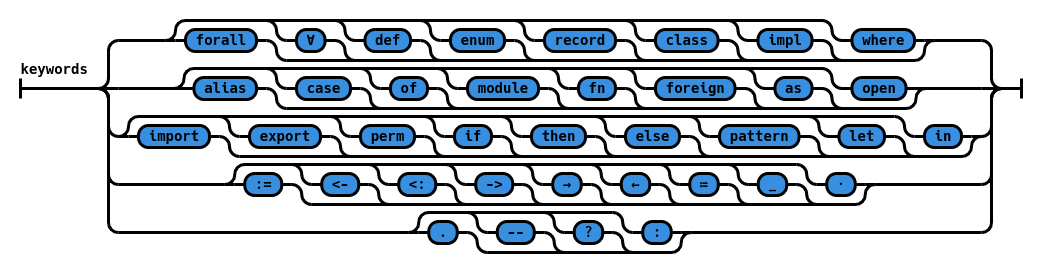
\includegraphics{zilch/lexicon/keywords}
  }
  \\
  \scalebox{.5}{
    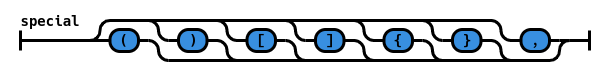
\includegraphics{zilch/lexicon/special}
  }
  \\
  \scalebox{.5}{
    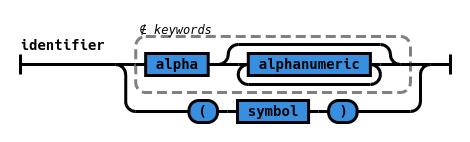
\includegraphics{zilch/lexicon/identifier}
  }

  \caption{Lexical units for identifiers.}
  \label{fig:zilch-grammar-lexical-identifiers-grammar}
\end{figure}

\subsection{Whitespaces}\label{subsec:zilch-grammar-lexical-whitespaces}

Whitespace tokens are basically word separators.
Because of that, comments are also counted as whitespaces, despite not really being an invisible sequence.
However, because of how mixfix operators are parsed, the sequence \verb|_--_...| corresponds to the two tokens \verb|<underscore>| and \verb|<comment _...>|, not \verb|<identifier _--_...>| (same goes for any mixfix operator that has \verb|--| as a backbone; but again, \verb|_--*_| \textit{is a valid operator}).

\begin{figure}[H]
  \centering

  \scalebox{.5}{
    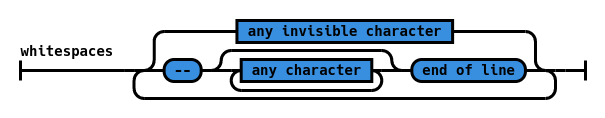
\includegraphics{zilch/lexicon/whitespaces}
  }

  \caption{Whitespace lexical units.}
  \label{fig:zilch-grammar-lexical-whitespaces-grammar}
\end{figure}

\subsection{Numerical tokens}\label{subsec:zilch-grammar-lexical-numbers}

There are two kinds of numerical tokens: integers and floating points.
While floating points are always written using decimal digits, integers may be written using decimal digits, octal digits (if prefixed by \verb|0o| or \verb|0O|), hexadecimal digits (if prefixed by \verb|0x| or \verb|0X|) or binary digits (if prefixed by \verb|0b| or \verb|0B|).
A floating point number must always have digits on both sides of the dot (i.e.\ it is impossible to write \verb|0.| as in other programming languages) because it could else be mistaken with the dot syntax.

\begin{figure}[H]
  \centering

  \scalebox{.5}{
    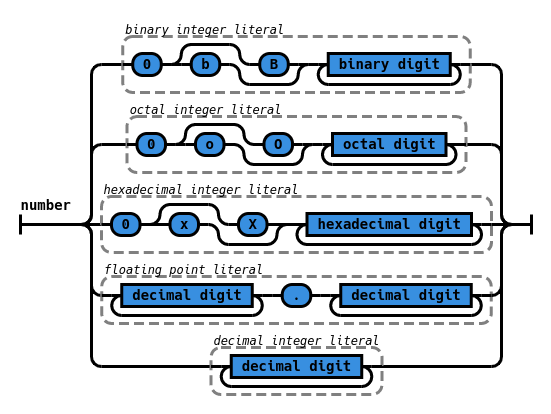
\includegraphics{zilch/lexicon/number}
  }

  \caption{Numeric lexical units.}
  \label{fig:zilch-grammar-lexical-numbers-grammar}
\end{figure}

\subsection{String and character literals}\label{subsec:zilch-grammar-lexical-strings}

Strings are arrays of characters.
However, because it is tedious to write such arrays, we provide syntactic sugar to make it easier.

String literals are enclosed in double quotes \verb|"|, and character literal are enclosed in single quotes \verb|'|.
They can contain any character (both graphical and whitespaces), but some characters may be easier to type.
These basically have ``shorthands'' defined as escape sequences, each defined in Table~\ref{table:zilch-grammar-lexical-strings-escapesequences}.
Note that, while double and single quotes may be escaped, these may not necessarily be in respectively character and string literals.

Multiple string literals directly next to each other (as in \verb|"abc" "def"|) are concatenated into one (so \verb|"abcdef"|).

\begin{figure}[H]
  \centering

  \scalebox{.5}{
    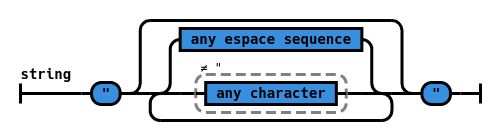
\includegraphics{zilch/lexicon/string}
  }
  \\
  \scalebox{.5}{
    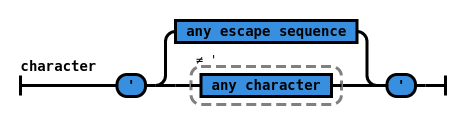
\includegraphics{zilch/lexicon/character}
  }

  \caption{String and character lexical units.}
  \label{fig:zilch-grammar-lexical-strings-grammar}
\end{figure}

\begin{table}[htb]
  \begin{tabularx}{\textwidth}{*{5}{Y}}
    \toprule
    \verb|\a| & \verb|\b| & \verb|\f| & \verb|\n| & \verb|\r| \\
    \verb|\t| & \verb|\v| & \verb|\\| & \verb|\"| & \verb|\'| \\
    \bottomrule
  \end{tabularx}

  \caption{All available escape sequences.}
  \label{table:zilch-grammar-lexical-strings-escapesequences}
\end{table}

\section{Expressions}\label{sec:zilch-grammar-expressions}

Expressions are the basic building block of Zilch.
\textit{Everything} is an expression, from simple arithmetic like \texttt{3 + 6} to complex \texttt{do} blocks.

Because of the presence of mixfix operators, it is harder to express a correct grammar.
For conciseness sake, the disambiguation of mixfix operators into their correct application is left to a non-described process that we will simply refer to as ``desugaring''\footnote{Desugaring basically transforms an expression into a corresponding simpler expression to analyse later. E.g. \texttt{if c then t else e} is transformed into the simpler application \texttt{if\_then\_else\_ c t e}.}.

\subsection{Lambda abstraction}\label{subsec:zilch-grammar-expressions-lambda}

Lambda abstractions allow creating ``in-place'' anonymous functions.
For example, both following alternatives are equivalent (because the lambda abstraction does not capture anything there):\\
\begin{minted}{\zilchlexer}
  -- Alternative 1
  def f(l: list u64): list u64 := map(fn(x) x * 2, l)
  -- Alternative 2
  def mapper(x: u64): u64 := x * 2
  def f(l: list u64): list u64 := map(mapper, l)
\end{minted}
\vspace*{\baselineskip}

\noindent However, these two are not quite equivalent:\\
\begin{minted}{\zilchlexer}
  -- Alternative 1
  def f(y: u64, l: list u64): list u64 := map(fn(x) x + y * 2, l)
  -- Alternative 2
  def mapper(y: u64)(x: u64): u64 := x + y * 2
  def f(y: u64, l: list u64): list u64 := map(mapper y, l)
\end{minted}
\vspace*{\baselineskip}

\noindent Note that lambda abstractions cannot be recursive on their own, they need to be bound using a \texttt{def} declaration.

There is also an alternative grammar for lambda abstractions, using wildcards abstractions.
Sometimes, you have to write \verb|reduce(fn(acc, e) acc + e, 0, list)|, but it would be far more pleasant if it could be written as in Haskell, i.e. \verb|reduce (+) 0 list|.
\verb|(+)| cannot unfortunately be written as is in Zilch.
This is why there are wildcard abstractions: it allows writing \verb|reduce(_ + _, 0, list)| (note the extra spaces around the operator, even though \verb|_+_| would have also worked just fine here) which makes it cleaner looking.
\verb|_ + _| is really syntactic sugar for \texttt{fn($x_0$) fn($x_1$) $x_0$ + $x_1$}.

A simple rule to convert wildcard abstractions to explicit lambda abstractions is the following: for each wildcard $\cdot_i$ in an expression \verb|e| (assuming from the left to the right), assign an unique identifier $u_i$ and replace the wildcard with it (also increment $i$). If $i \neq 0$ at the end, then replace \verb|e| with the lambda abstraction \texttt{fn($u_0$, \ldots, $u_i$) e[$\cdot_0$\textbackslash$u_0$, \ldots, $\cdot_i$\textbackslash$u_i$]}.
Some examples are given in Table~\ref{table:zilch-grammar-expressions-lambda-translatewildcard}.

\begin{figure}[H]
  \centering

  \scalebox{.5}{
    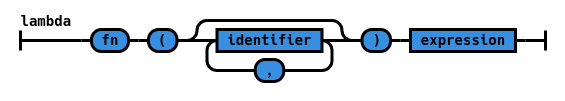
\includegraphics{zilch/expression/lambda}
  }

  \caption{Grammar for lambda abstractions.}
  \label{fig:zilch-gramma-expressions-lambda-grammar}
\end{figure}

\begin{table}[htb]
  \begin{tabularx}{\textwidth}{YcY}
    \toprule
    From & \multirow{5}{*}{\textbf{$\rightsquigarrow$}} & To \\
    \midrule
    \verb|_ + 1| && \verb|fn(x0) x0 + 1| \\
    \verb|f(_)| && \verb|fn(x0) f(x0)| \\
    \verb|f(_ * 2)| && \verb|f(fn(x0) x0 * 2)| \\
    \verb|f(_ * 2, _)| && \verb|fn(x0) f(fn(x1) x1 * 2, x0)| \\
    \bottomrule
  \end{tabularx}

  \caption{Some examples of wildcard abstraction translation.}
  \label{table:zilch-grammar-expressions-lambda-translatewildcard}
\end{table}

\subsection{Conditional}\label{subsec:zilch-grammar-expressions-conditional}

Conditional expressions allow selecting an expression based off the value of a condition.
However, it only works as a binary selector.
If n-ary selectors are needed, chaining \texttt{if}s is the only solution.

\begin{figure}[H]
  \centering

  \scalebox{.5}{
    
\includegraphics{zilch/expression/conditional}
  }

  \caption{Grammar for conditional expressions.}
  \label{fig:zilch-gramma-expressions-conditional-grammar}
\end{figure}

\subsection{Do block}\label{subsec:zilch-grammar-expressions-do}

Do blocks are expressions allowing variable bindings, much-like the usual \texttt{let \ldots in \ldots} from functional programming (both are really the same thing in fact, but a prettier approach was taken with Zilch; chaining \texttt{let-in}s is not necessarily very pleasant to the eye).
Note that a do block \textbf{must} finish with a simple expression, used as the return value of the whole block.

\begin{figure}[H]
  \centering

  \scalebox{.5}{
    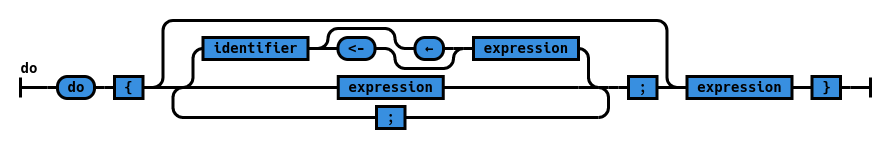
\includegraphics{zilch/expression/do}
  }

  \caption{Grammar for do blocks.}
  \label{fig:zilch-gramma-expressions-do-grammar}
\end{figure}

\subsection{Pattern matching}\label{subsec:zilch-grammar-expressions-case}

Pattern matching is achieved through the use of a \texttt{case} expression.

\begin{figure}[H]
  \centering

  \scalebox{.5}{
    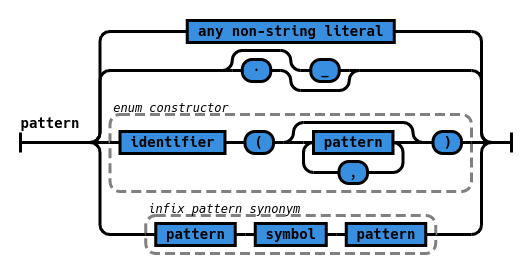
\includegraphics{zilch/expression/pattern}
  }\\
  \scalebox{.5}{
    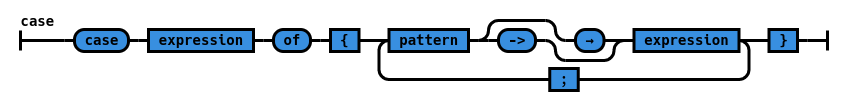
\includegraphics{zilch/expression/case}
  }

  \caption{Grammar for case expressions.}
  \label{fig:zilch-gramma-expressions-case-grammar}
\end{figure}

\subsection{Record literals}\label{subsec:zilch-grammar-expressions-record}

Record literals allow constructing records in the same fashion as in e.g.\ C.

\begin{figure}[H]
  \centering

  \scalebox{.5}{
    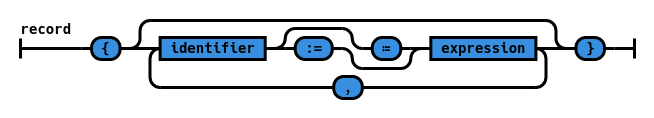
\includegraphics{zilch/expression/record}
  }

  \caption{Grammar for record literals.}
  \label{fig:zilch-gramma-expressions-record-grammar}
\end{figure}

\subsection{Mixfix operators}\label{subsec:zilch-grammar-expressions-mixfix}

Mixfix operators allow expressing n-ary operators.
For example, in Haskell you can only define infix operators (that is, any operator of the form \verb|_<op>_|) and has a limited support for unary operators (prefix and postfix, \verb|<op>_| and \verb|_<op>|).
Yet there are other kinds of operators.
Operators may also be closed (\verb|<op>_<op>|), and contain more than two holes: \verb|if_then_else_| is a great example of ternary prefix operator.

Mixfix disambiguation will not be covered in this document, because of how difficult it is.
However, Ulf Norell's paper~\cite{mixfix-operators} about parsing mixfix operators is a great resource for this.

Note that, while \verb|_| is allowed in identifiers, having one in a mixfix backbone may not yield any parse result, because \verb|_| represents a hole when declaring the operator.
Therefore, the operator \verb|_+_| cannot be used like \verb|0 _+_ 1| or \verb|0 +_ 1| (both give parse errors), but it may be used as a standard function application like \verb|_+_(0, 1)|.

\begin{figure}[H]
  \centering

  \scalebox{.5}{
    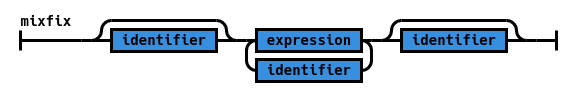
\includegraphics{zilch/expression/mixfix}
  }

  \caption{Grammar for mixfix operators.}
  \label{fig:zilch-grammar-expressions-mxifix-grammar}
\end{figure}

\subsection{Variables, typed holes and literals}\label{subsec:zilch-grammar-expressions-basicexpr}

\begin{figure}[H]
  \centering

  \scalebox{.5}{
    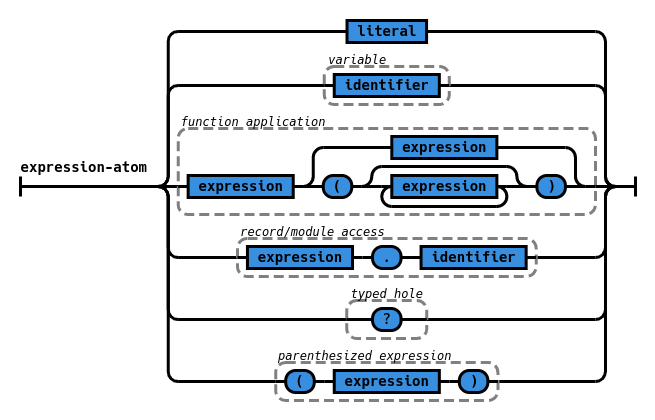
\includegraphics{zilch/expression/atom}
  }

  \caption{Grammar for expression atoms.}
  \label{fig:zilch-grammar-expressions-atom-grammar}
\end{figure}

\section{Types}\label{sec:zilch-grammr-types}

Types lie at the same level as expressions, but are put in a separate section for comprehensiveness sake.
An expression \verb|e| is said to be of type \verb|t| if evaluating it yields (or at least is supposed to) any value in the set \verb|t|.

Wildcard abstractions are only allowed in \verb|impl| blocks, despite being a general type, and follow the same desugaring rules as their expression-level counterparts (see Table~\ref{table:zilch-grammar-expressions-lambda-translatewildcard} for some examples; replace \verb|fn| with \verb|Fn| and you have the type-level counterparts).
Any other type can be used anywhere.

\begin{figure}[H]
  \centering

  \scalebox{.5}{
    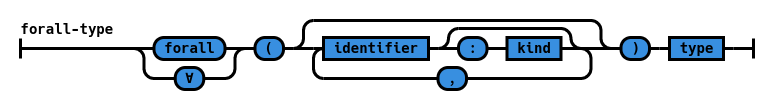
\includegraphics{zilch/types/forall}
  }\\
  \scalebox{.5}{
    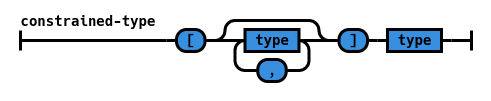
\includegraphics{zilch/types/constrained}
  }\\
  \scalebox{.5}{
    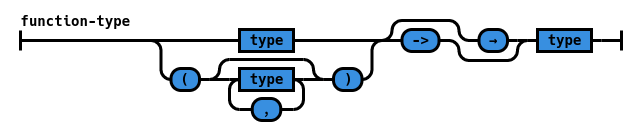
\includegraphics{zilch/types/function}
  }\\
  \scalebox{.5}{
    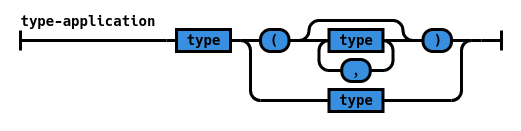
\includegraphics{zilch/types/application}
  }\\
  \scalebox{.5}{
    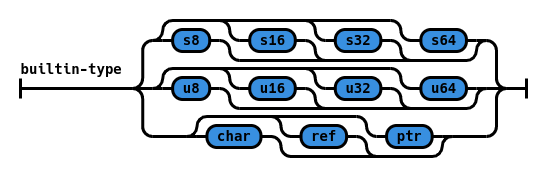
\includegraphics{zilch/types/builtin}
  }\\
  \scalebox{.5}{
    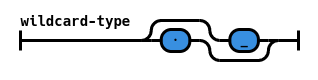
\includegraphics{zilch/types/wildcard-abstraction}
  }

  \caption{Grammar for types.}
  \label{fig:zilch-grammar-types-grammar}
\end{figure}

\section{Declarations}\label{sec:zilch-grammar-declarations}

A Zilch module is composed of zero or more declarations.
There are 5 possible declarations:
\begin{itemize}
  \item Type class declaration
  \item Type class implementation
  \item New type definition
  \item Value definition
  \item Fixity declaration
\end{itemize}

\noindent Each of them will be syntactically described in this section.

\subsection{Value definition}\label{subsec:zilch-grammar-declarations-value}

\begin{figure}[H]
  \centering

  \scalebox{.5}{
    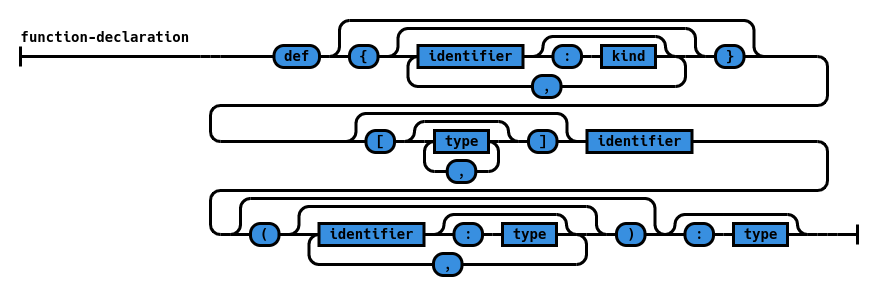
\includegraphics{zilch/toplevel/function-declaration}
  }\\
  \scalebox{.5}{
    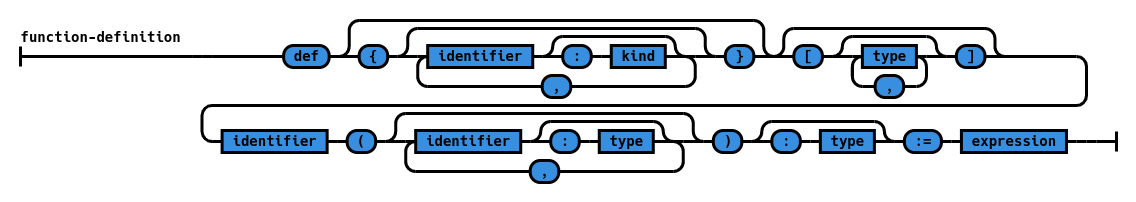
\includegraphics{zilch/toplevel/function-definition}
  }

  \caption{Grammar for value declarations.}
  \label{fig:zilch-grammar-declarations-value-grammar}
\end{figure}

\subsection{Operator fixity declaration}\label{subsec:zilch-grammar-declarations-fixity}

\begin{figure}[H]
  \centering

  \scalebox{.5}{
    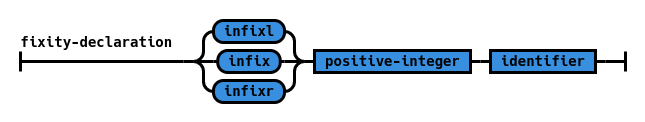
\includegraphics{zilch/toplevel/fixity-declaration}
  }

  \caption{Grammar for operator fixity declarations.}
  \label{fig:zilch-grammar-declarations-fixity-grammar}
\end{figure}

\subsection{New type definition}\label{subsec:zilch-grammar-declarations-type}

\begin{figure}[H]
  \centering

  \scalebox{.5}{
    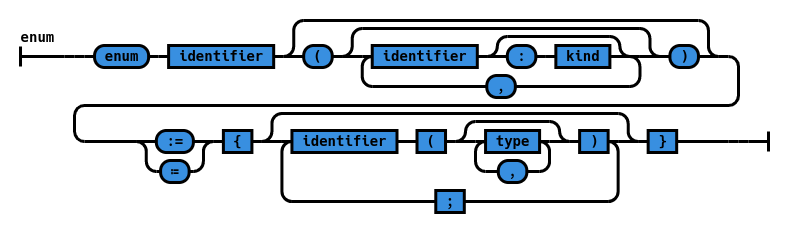
\includegraphics{zilch/toplevel/enum-definition}
  }\\
  \scalebox{.5}{
    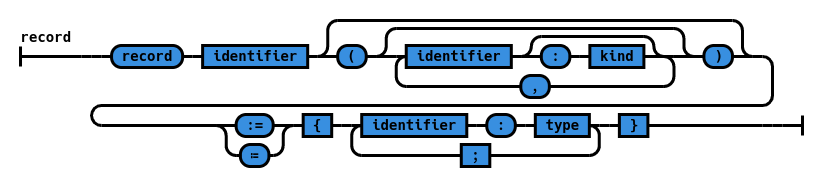
\includegraphics{zilch/toplevel/record-definition}
  }\\
  \scalebox{.5}{
    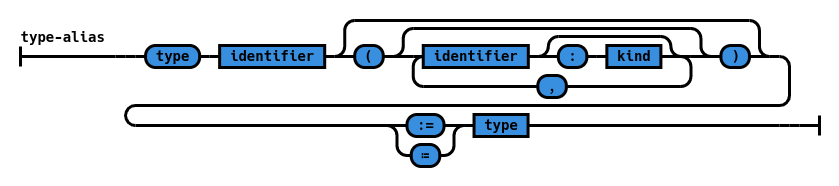
\includegraphics{zilch/toplevel/alias-definition}
  }

  \caption{Grammar for new type definitions.}
  \label{fig:zilch-grammar-declarations-type-grammar}
\end{figure}

\subsection{Type class declaration}\label{subsec:zilch-grammar-declarations-typeclass}

\begin{figure}[H]
  \centering

  \scalebox{.5}{
    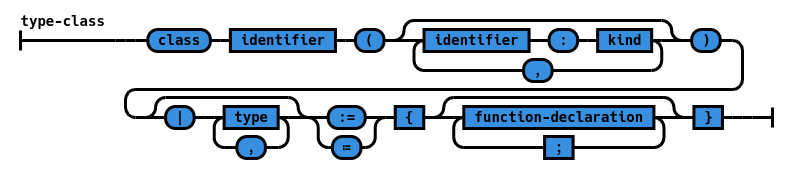
\includegraphics{zilch/toplevel/typeclass-declaration}
  }

  \caption{Grammar for type-class declarations.}
  \label{fig:zilch-grammar-declarations-typeclass-grammar}
\end{figure}

\subsection{Type class implementation}\label{subsec:zilch-grammar-declarations-implementation}

\begin{figure}[H]
  \centering

  \scalebox{.5}{
    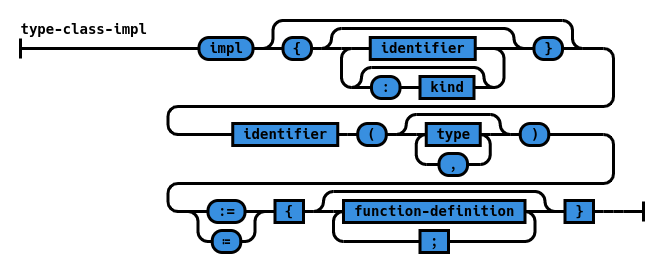
\includegraphics{zilch/toplevel/implementation-definition}
  }

  \caption{Grammar for type-class implementations.}
  \label{fig:zilch-grammar-declarations-implementation-grammar}
\end{figure}
